\documentclass[tikz,border=5pt]{standalone}
% ============================================================
%  style.tex
%  Style commun pour les graphes de fonctions et d'intégrales
%  Usage : \input{style.tex}  (à placer après \documentclass)
% ============================================================

\usepackage{pgfplots}
\pgfplotsset{compat=1.18}
\usepackage[T1]{fontenc}
\usepackage{amsmath,amsfonts}
\usepackage{xcolor}
\usetikzlibrary{patterns}
\usepgfplotslibrary{fillbetween}

% ---- Couleurs standard ----
\colorlet{monGris}{black!45}   
\colorlet{monBleu}{blue!60}  

% ============================================================
%  Styles TikZ (\tikzset) : tout ce qui touche à l'apparence
%  (couleurs, épaisseurs, hachures, position des étiquettes...)
%  -> utilisables aussi bien sur \node, \draw, \addplot, etc.
% ============================================================
\tikzset{
  % Courbe "secondaire" en nuance de gris (tracé + étiquette)
  courbe/.style={thick},
  % Hachures
  hachure/.style={
    pattern=north east lines,
    pattern color=#1,
    draw=none,
    samples=100,
    /pgfplots/forget plot,
  },
  hachure/.default=black,
}

% ============================================================
%  Style pgfplots (\pgfplotsset) : options propres à l'environnement axis
%  (repère orthonormé, ticks, épaisseur des axes...)
%  -> ces clés n'existent que dans /pgfplots/, \tikzset ne peut pas les définir.
% ============================================================
\pgfplotsset{
    axes/.style={
    axis lines=middle,
    axis equal image,               % repère orthonormé
    thick,                          % épaisseur des axes et courbes
    samples=200,
  }
}


\begin{document}
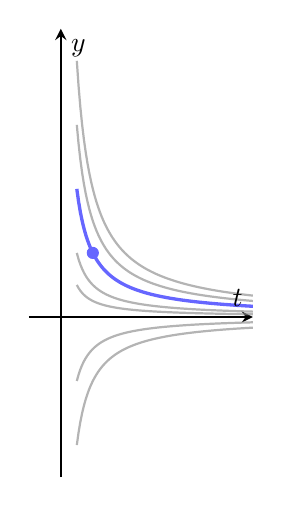
\begin{tikzpicture}
\begin{axis}[
    axes,
    xlabel={$t$},
    ylabel={$y$},
    xmin=-1, xmax=6,
    ymin=-5, ymax=9,
    domain=0.5:6,
    samples=100,
    xtick=\empty,
    ytick=\empty,
]

% Courbes intégrales de ty' + y = 0 (exemple 7.1) : y = c/t, c \in R
% (sur ]0,+\infty[, elles ne se coupent jamais)
\foreach \c in {-2,-1,0.5,1,3,4} {
    \addplot[courbe, monGris, opacity=0.65] {\c/x};
}

% La courbe intégrale passant par le point de Cauchy (1,2) : y = 2/t
\addplot[courbe, monBleu, very thick, domain=0.5:6] {2/x};


% Point de Cauchy (1,2)
\fill[monBleu] (axis cs:1,2) circle (2.2pt);


\end{axis}
\end{tikzpicture}
\end{document}
